\def \eng #1{\foreignlanguage{english}{#1}}

\textbf{Цель работы.}
%
\begin{enumerate}
	\item Практическое изучение теоремы о дискретизации на основе задачи цифрового ввода аналоговых сигналов с помощью интерфейсной платы и их последующей цифровой обработки.
    \item Ознакомление с методами восстановления изображений по проекциям.
\end{enumerate}

\textbf{Аппаратура.} Лабораторный макет \enquote{томограф}, источник питания, интерфейсная плата АЦП, персональный компьютер.

\textbf{Содержание работы.} Эмуляция работы томографа. Оцифровка проекций объекта, закрепленного в установке, с помощью АЦП, расположенного на интерфейсной плате. Восстановление двумерного изображения объекта по двум его ортогональным проекциям.

\section{Минимальные теоретические сведения}

\subsection{Описание лабораторной работы}

Одним из перспективных направлений методов компьютерной диагностики является метод компьютерной томографии. Буквально, слово \enquote{томография} означает послойное исследование объектов. В данной работе методы компьютерной томографии показываются на примере восстановления двумерного объекта по двум его одномерным проекциям.

Получение одномерных проекций производится путем многократного просвечивания пластинки по параллельным прямым узконаправленным световым пучком, который после прохождения через пластинку попадает на фотодиод.

\subsection{Описание лабораторного макета}

Установка (\autoref{fig:maket}) состоит из следующих функциональных узлов:

\begin{figure}[h]%
    \centering
    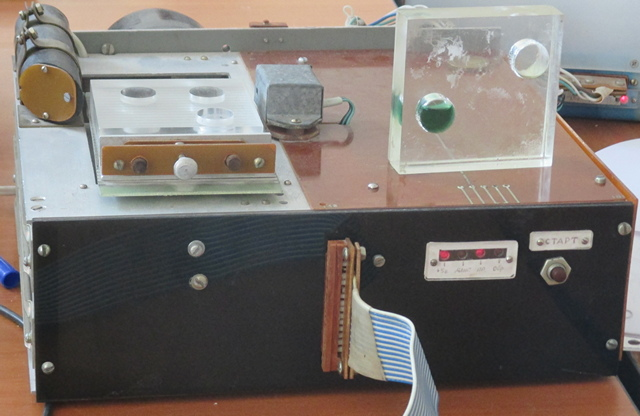
\includegraphics[width=0.8\textwidth]{maket}%
    \caption[]{Внешний вид лабораторного макета и томографируемых объектов}%
    \label{fig:maket}%
\end{figure}

\begin{enumerate}
\item подвижной платформы с укрепленным на ней объектом исследования;
\item расположенных по обе стороны от платформы неподвижных точечного источника излучения (светодиода) и приемника излучения (фотодиода);
\item устройства перемещения платформы, состоящего из реверсивного двигателя, управляемого триггерной схемой для обеспечения возвратно-поступательного перемещения платформы, и концевых датчиков достижения платформой крайних точек;
\item аналого-цифрового преобразователя (АЦП), преобразующего интенсивность принятого фотодиодом светового излучения в 10-разрядный цифровой код;
\item устройства ввода-вывода, представляющего собой плату, установленную в компьютер, и предназначенную для программного управления устройством перемещения платформы и ввода цифрового кода в компьютер.
\end{enumerate}

Управление установкой, обработку полученных данных и построение геометрических проекций исследуемого объекта осуществляется с помощью компьютера серии \eng{IBM PC AT}.

Пластинка движется между светодиодом и фотодиодом, при этом пучок, прошедший через пластинку, попадает на фотоприемник, который фиксирует его интенсивность. Триггерная схема, управляющая двигателем, при нажатии кнопки \enquote{Старт} запускает его для снятия проекции исследуемого предмета, а при достижении конца диапазона движения переключает двигатель на обратный ход. Когда платформа доезжает до начального положения, двигатель отключается, и установка ждет следующего нажатия кнопки \enquote{Старт}. Макет установки передает в компьютер информацию о текущем состоянии установки: движется ли она, в каком направлении, готов ли цифровой сигнал для передачи.

Таким образом, при поступательном движении подвижной платформы с установленным на ней объектом исследования через световой пучок проходит весь объект, и в компьютере формируется массив данных, соответствующий степени поглощения каждого элементарного объема объекта исследования. При достижении платформой конечного положения, определяющегося датчиком конечного положения, компьютер производит реверс двигателя, и платформа совершает возвратное движение до начального положения. Затем объект исследования устанавливается на платформе под другим углом к направлению движения, и установка запускается снова. Таким образом, после двух проходов в памяти компьютера имеются два массива данных, соответствующих степеням поглощения света каждым элементарным объемом в различных ракурсах.

Интерфейсная плата является восьмиразрядной и использует два порта в адресном пространстве компьютера: порт управления и порт данных. Кодограммы обмена приведены в техническом описании установки.

\subsection{Математическая модель}

При движении пластинки между источником и приемником излучения пучок света, прошедший через нее, попадает на фотоприемник, который фиксирует его интенсивность. Если принять интенсивность луча, прошедшего через пластинку из чистого оргстекла, за $I_0$, а фотодиод при некотором положении пластинки зарегистрировал интенсивность $I_i$, то

\begin{equation}\label{eq:i0ii}
    \frac{I_i}{I_0} = e^{-a_i} ,
\end{equation}

где $a_i$~--- интегральный показатель поглощения, то есть

\begin{equation}\label{eq:ai}
    a_i = \sum\limits_j\rho_{ij} .
\end{equation}

Логарифмированием обеих частей выражения \autoref{eq:i0ii} и подстановкой $a_i$ из выражения \autoref{eq:ai} получаем

\begin{equation}
    a_i = \log\frac{I_0}{I_i} ,
        \quad \text{или} \quad
    \sum\limits_j\rho_{ij} = \log\frac{I_0}{I_i} .
\end{equation}

Таким образом, моделируемый объект представляется в виде матрицы $\rho_{ij}$, где каждый элемент хранит значение оптической плотности в соответствующей точке пластинки, а $a_i$ представляет собой сумму элементов этой матрицы по одной линии (вертикали или горизонтали).

Для восстановления изображения по его проекциям в работе используется метод \enquote{обратной тени} (\eng{back-projection method}) в простейшей его постановке для двух ортогональных проекций изображения. Далее приводится краткое изложение сути метода.

\begin{enumerate}
\item [Шаг 0.] Пусть $S_i = \sum\limits_{j=0}^{N-1}\rho_{ij}$ и $C_j = \sum\limits_{i=0}^{N-1}\rho_{ij}$~--- две ортогональные проекции изображения.
\item [Шаг 1.] Начальное приближение: $\rho^0_{ij} = \flatfrac{S_i}{N}$.
\item [Шаг 2.] $\rho^{k+1/2}_{ij} = \rho^k_{ij} \flatfrac{C_j}{C^k_j}$, где $C^k_j = \sum\limits_{i=0}^{N-1}\rho_{ij}$.
\item [Шаг 3.] $\rho^{k+1}_{ij} = \rho^{k+1/2}_{ij} \flatfrac{S_i}{S^k_i}$, где $S^k_i = \sum\limits_{j=0}^{N-1}\rho^{k+1/2}_{ij}$.
\end{enumerate}

Шаги 2-3 выполняются до тех пор, пока изменение в числовых рядах $S^k_i$ и $C^k_j$ от итерации к итерации не станет достаточно малым.

\section{Результаты и их обсуждение}

\subsection{Интерфейс программы управления}

Для организации работы с устройством была разработана программа с графическим интерфейсом (\autoref{fig:app}).

\begin{figure}[h]%
\centering
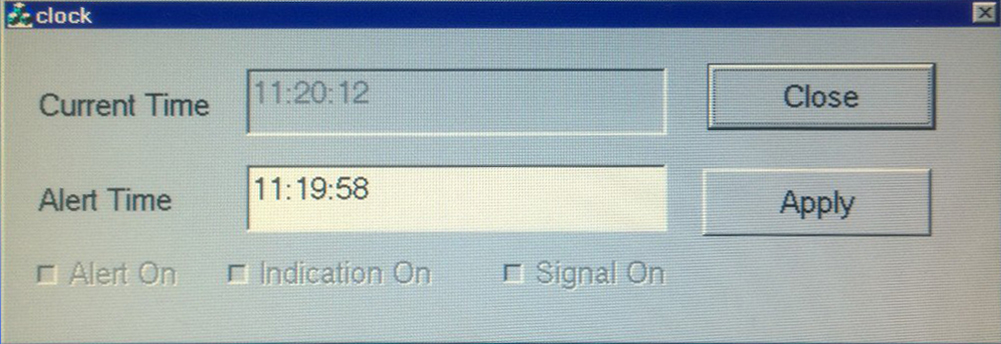
\includegraphics[width=0.8\textwidth]{app}%
\caption[]{Главное окно программы}%
\label{fig:app}%
\end{figure}

Программа в фоновом режиме следит за состоянием аппаратуры (наличие питания, движение платформы вперед/назад и т.п.). При запуске платформы с управляющей панели лабораторного макета программа начинает подготовку к снятию проекции изображения. Выбор номера проекции (первая или вторая) оставляется за оператором программы.

После снятия проекционных данных обеих проекций возможно получить восстановленное двумерное изображение путем нажатии соответствующей кнопки.

Операторский интерфейс программы предусматривает возможность выгрузки в файл и загрузки из файла проекционных данных.

\subsection{Архитектура программы управления}

Программа управления была написана в среде \eng{Microsoft Visual Studio 6.0} на языке \eng{\tt c++} с использованием библиотеки классов \eng{MFC} (\eng{Microsoft Foundation Classes}).

Для инкапсуляции низкоуровневого программного интерфейса устройства и проведения работы по обработке оцифрованных были описаны и реализованы два интерфейса (абстрактных класса):
%
\begin{enumerate}
	\item \eng{\tt CDevice} --- инкапсулирует чтение регистра состояния аппаратуры, инициализацию режима снятия проекционных данных и, собственно, снятие проекционных данных.
	\item \eng{\tt CImageReconstuctor} --- инкапсулирует алгоритм восстановления по проекциям двумерного изображения.
\end{enumerate}

Объект класса \eng{\tt CDevice} создает фоновый вычислительный поток, в котором происходит слежение за состоянием аппаратуры. При каждом изменении состояния аппаратуры, по готовности проекционных данных и при ошибке снятия проекционных данных объект класса через функцию обратной связи оповещает главное окно приложения.

При переходе аппаратуры в состояние движения платформы вперед начинается замер времени до момента изменения направления движения платформы. Измеренное время используется для определения временн\'{о}го периода дискретизации при снятии проекции. Период дискретизации вычисляется из условия обеспечения необходимой пространственной частоты дискретизации. Она, в свою очередь, определяется максимальной частотой в спектре проекции изображения, т.е. в конечном счете установленным в макете объектом.

После начала обратного движения платформы начинается процесс снятия проекционных данных. Через рассчитанный интервал (период дискретизации) производится запуск АЦП и получение отсчета данных, которые запоминаются и по окончании движения платформы передаются главному окну программы через функцию обратной связи.

Для восстановления двумерного изображения используется объект класса \eng{\texttt{\justify CImageReconstuctor}}.

Результаты снятия проекций и результат восстановления изображения по проекциям отображаются в главном окне программы.

\section{Выводы}

В ходе работы была реализована программа для организации работы с лабораторным макетом \enquote{томограф}.

Была практически изучена теорема о дискретизации на основе задачи цифрового ввода аналоговых сигналов с помощью интерфейсной платы и их последующей цифровой обработки.